\section{Astrophysics}

\subsection{astronomical distances}

\subsubsection{unit of length in astronomy}

distances between stars and galaxies in the universe are very large

so it is more convenient to introduce alternative units of measurement for lengths

\cmt astronomical unit (AU)

an astronomical unit is the average distance between the Earth and the Sun
\begin{equation*}
    1 \text{ AU} \approx 1.50 \times 10^{11} \text{ m}	
\end{equation*}

\cmt light-year (ly)

a light-year is the distance that light can travel in one year
\begin{equation*}
	1 \text{ ly} = 3.00\times10^8 \mps \times 365 \times 24 \times 3600 \text{ s}  \approx 9.46 \times 10^{15} \text{ m}
\end{equation*}

\cmt parsec (pc) ($\ast$)

one parsec is the distance at which 1 AU subtends an angle of 1 arcsec or $\frac{1^\circ}{3600} $
\begin{equation*}
	1 \text{ pc} = \frac{1.50 \times 10^{11} \text{ m}}{\frac{1^\circ}{3600} \times \frac{2\pi}{360^\circ}} \approx 3.09 \times 10^{16} \text{ m}
\end{equation*}


\subsubsection{luminosity}\index{luminosity}

\begin{ilight}
	\keypoint{luminosity} (L) of an object is the total power emitted by this object
\end{ilight}

\cmt unit for luminosity: $[L] = \text{W} = \text{J s}^{-1}$

\cmt luminosity of a star depends on its surface temperature and its size

\titem temperature $T \up \ra L \up$

\titem stellar radius $R \up \ra L \up$

\subsubsection{radiant flux intensity}\index{radiant flux intensity}

\begin{ilight}
	\keypoint{radiant flux intensity} ($F$) is defined as the radiant power passing through a surface per unit area at right angles
\end{ilight}

\cmt unit for radiant flux intensity: $[F] = \text{W m}^{-2}$

\cmt $F$ measures \emph{observed} intensity, i.e., $F$ gives \emph{apparent brightness} of the object

\cmt $F$ depends on distance from the emitting source

if radiation through space is uniform with no absorption, then: $\boxed{F=\frac{L}{4 \pi d^2}}$

\example{The luminosity of the sun is approxiamately $3.86\times10^{26}$ W. Given that the distance between the earth and the sun is about $1.5\times10^{11}$ m, what is the theoretical power of a space probe that has a solar pane of an area of 40 m$^2$? }

\sol radiant flux intensity: $F = \frac{L}{4\pi d^2} = \frac{3.86\times10^{26}}{4\pi\times(1.5\times10^{11})^2} \approx 1370 \text{ W m}^{-2}$

power input: $P = F A = 1370 \times 40 \approx5.46 \times 10^{4} \text{ W}$ \eoe

\example{The radiant flux intensity due to the sun at the position of the earth is about 2.3 times greater than that at the position of the Mars. Given that the distance between the earth and the sun is about $1.5\times10^{11}$ m, how far is the Mars from the sun?}

\solc \begin{equation*}
	F \propto \frac{1}{d^2} \RA \frac{F_E}{F_M} = \frac{d_M^2}{d_E^2} \RA \frac{d_M^2}{d_E^2} = 2.3 \RA d_M = {\sqrt{2.3}}\times1.5\times10^{11} \approx 2.3\times10^{11} \text{ m} \teoe
\end{equation*}

\subsubsection{standard candles}\index{standard candle}

\begin{ilight}
	astronomical objects of known luminosity are called \keypoint{standard candles}
\end{ilight}

for a particular star, say $X$, we can look for a standard candle in the same galaxy

radiant flux intensity $F$ of the standard candle can be measured, and its luminosity $L$ is also known, so its distance can be found using: $d = \sqrt{\frac{L}{4\pi F}}$

distance of star $X$ is about same as distance of standard candle, as they are in same galaxy

this is how we determine the distance of stars by the use of \emph{standard candles}


\newpage

among the many types of standard candles you need to know two in this course:

\titem cepheid variables

\titem supernovae

\subsubsection*{cepheid variables}\index{standard candle!cepheid variable}

cepheid variables are stellar objects whose brightness varies periodically\footnote{The variation in the stellar brightness is related to the mass of the cepheid variable. When the star contracts, its core temperature increases, this boosts the rate of nuclear reaction so radiation pressure increases to push the stellar matter outwards against the gravity. But as the star expands, its temperature drops so its radiation pressure lowers, the gravitational attraction would tend to pull the stellar matter inwards. The period of this feedback loop between the gravitational pull and the nuclear reaction taking place in the star depends on the mass of the star, and the mass of the star determines a number of the star's features including its luminosity. Therefore, if we know the period of the brightness fluctuations, we can know about the star's mass and hence its luminosity.}

once we know period of variation in brightness, luminosity of the star can be predicted

\example{One cepheid variable has a radiuant flux intensity of $1.4 \times 10^{-16} \text{ W m}^{-2}$. It is known to have a luminosity of $1.0 \times 10^{30} \text{ W}$. Find the distance of this star in light-years.}

\yskip

\solc\begin{equation*}
	F = \frac{L}{4\pi d^2} \RA d = \sqrt{\frac{L}{4\pi F}} = \sqrt{\frac{1.0 \times 10^{30}}{4\pi \times 1.4 \times 10^{-16}}} \approx 2.4 \times 10^{22} \text{ m} = \frac{2.4 \times 10^{22}}{9.46\times10^{15} } \text{ ly} \approx 2.5\times10^6 \text{ ly} \teoe
\end{equation*}

\subsubsection*{supernovae}\index{standard candle!supernova}

luminosity of supernovae is known to be constant\footnote{To be more precise, Type Ia supernovae explosions are found to have a consistent luminosity. These events are believed to occur when a white dwarf accretes matter until its mass exceeds a critical value, known as the Chadellaskar limit. By then its gravitational attraction can no longer be overcome by the degeneracy pressure, the star collapses and explodes. There is also Type II supernovae explosions, these occur when a star of very large mass runs out of its nuclear fuel. Radiation pressure cannot be maintained, so the star collapses rapidly towards its centre under gravity.}

\cmt supernovae are extremely luminous, so suitable for measuring very large distances

\question{(a) Type 1a supernovae have luminosities at the order of $10^{36} \text{ W}$ (approximately 5 billions of the luminosity of the sun). If the sun undergoes a supernova explosion, find the radiant flux intensity measured on earth. (b) It is estimated that the Hiroshima bomb and the Nagasaki bomb (the two nuclear bombs dropped on Japan during the World War II) released a total energy of around 100 TJ. Suppose a similar nuclear bomb completely explodes at a distance of 50 m from your home in a period of one second, what radiant flux intensity do you measure? (c) Compare the two results, which event would appear brighter?}




\subsection{spectrum of stars}

any object at a particular temperature $T$ emits electromagnetic radiation

radiation emitted by the object spreads into a continuous range of wavelengths $\lambda$

total intensity and typical wavelength emitted depend influentially on temperature $T$

for example, human body ($\sim 300 \text{ K}$) emits infra-red, cooking fire ($\sim 1000 \text{ K}$) emits visible red

stars also emit radiation with a range of wavelengths, giving rise to a characteristic spectrum

we can learn a lot about the properties of the star by looking at its spectrum

\subsubsection{black body radiation}\index{black body radiation}

theoretically, stars can be modelled as black body emitters, whose emission spectrum at a particular temperature $T$ can be precisely predicted

\begin{ilight}
	a \keypoint{black body} is an idealised object that absorbs all incident radiation
\end{ilight}

\cmt intensity spectrum of black body radiation has the following features:

\titem for given temperature, intensity tends to zero at very short or very long wavelengths

\titem as temperature increases, peak intensity occurs at shorter wavelength ($T\up \ra \lambda_\text{max}\down$)

\titem for any $\lambda$, intensity increases with temperature ($T\up \ra I\up$)


\begin{figure}[ht]
	\centering
	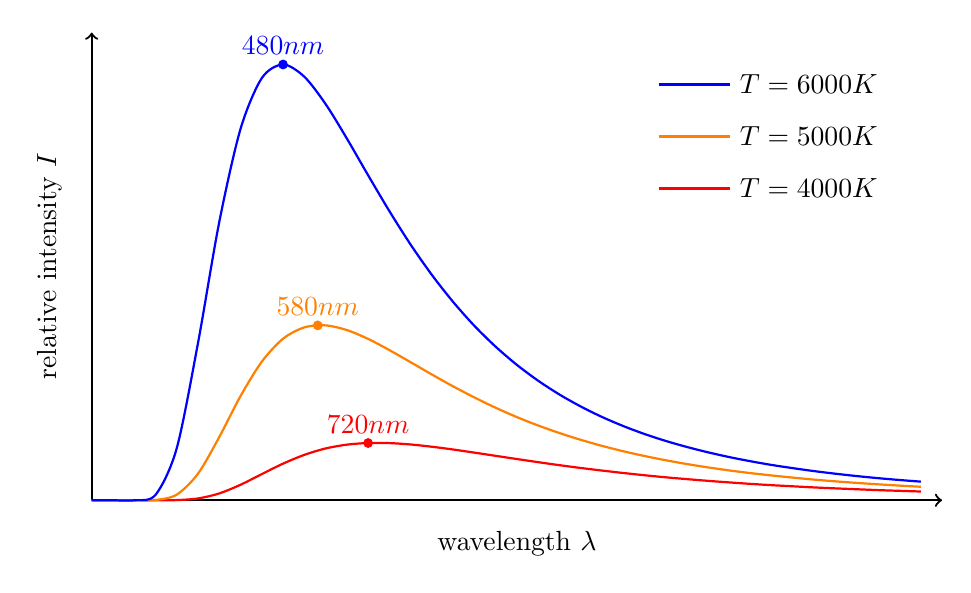
\begin{tikzpicture}[xscale=9, yscale=1.1]
	\draw [thick, ->] (0,0) --(1.2,0);
	\node at (0.6, -0.5) {wavelength $\lambda$};
	\draw [thick, ->] (0,0) --(0,5.4);
	\node[rotate=90] at (-0.06, 2.7) {relative intensity $I$};
	\draw [red, thick] plot [smooth] coordinates {(0, 0) (0.030, 0.000) (0.060, 0.000) (0.090, 0.000) (0.120, 0.002) (0.150, 0.021) (0.180, 0.079) (0.210, 0.179) (0.240, 0.302) (0.270, 0.423) (0.300, 0.524) (0.330, 0.598) (0.360, 0.642) (0.390, 0.661) (0.420, 0.660) (0.450, 0.644) (0.480, 0.618) (0.510, 0.586) (0.540, 0.550) (0.570, 0.513) (0.600, 0.476) (0.630, 0.440) (0.660, 0.405) (0.690, 0.373) (0.720, 0.343) (0.750, 0.315) (0.780, 0.289) (0.810, 0.265) (0.840, 0.244) (0.870, 0.224) (0.900, 0.206) (0.930, 0.189) (0.960, 0.174) (0.990, 0.161) (1.020, 0.148) (1.050, 0.137) (1.080, 0.127) (1.110, 0.117) (1.140, 0.109) (1.170, 0.101) };
	\draw[red, fill] (0.390, 0.661) ellipse(0.006 and 0.05) node[above]{$720 \text{ nm}$};
	\draw [orange, thick] plot [smooth] coordinates {(0, 0) (0.030, 0.000) (0.060, 0.000) (0.090, 0.003) (0.120, 0.065) (0.150, 0.307) (0.180, 0.730) (0.210, 1.203) (0.240, 1.600) (0.270, 1.865) (0.300, 1.996) (0.330, 2.019) (0.360, 1.965) (0.390, 1.863) (0.420, 1.734) (0.450, 1.594) (0.480, 1.452) (0.510, 1.315) (0.540, 1.187) (0.570, 1.068) (0.600, 0.960) (0.630, 0.863) (0.660, 0.776) (0.690, 0.698) (0.720, 0.628) (0.750, 0.566) (0.780, 0.511) (0.810, 0.462) (0.840, 0.418) (0.870, 0.379) (0.900, 0.344) (0.930, 0.313) (0.960, 0.286) (0.990, 0.261) (1.020, 0.238) (1.050, 0.218) (1.080, 0.200) (1.110, 0.184) (1.140, 0.169) (1.170, 0.156)  };
	\draw[orange, fill] (0.319, 2.019) ellipse(0.006 and 0.05) node[above]{$580 \text{ nm}$};
	\draw [blue, thick] plot [smooth] coordinates {(0, 0) (0.030, 0.000) (0.060, 0.000) (0.090, 0.062) (0.120, 0.601) (0.150, 1.816) (0.180, 3.213) (0.210, 4.288) (0.240, 4.874) (0.270, 5.031) (0.300, 4.890) (0.330, 4.575) (0.360, 4.177) (0.390, 3.753) (0.420, 3.339) (0.450, 2.952) (0.480, 2.602) (0.510, 2.290) (0.540, 2.014) (0.570, 1.773) (0.600, 1.563) (0.630, 1.380) (0.660, 1.221) (0.690, 1.083) (0.720, 0.962) (0.750, 0.857) (0.780, 0.765) (0.810, 0.685) (0.840, 0.615) (0.870, 0.553) (0.900, 0.498) (0.930, 0.450) (0.960, 0.407) (0.990, 0.370) (1.020, 0.336) (1.050, 0.306) (1.080, 0.279) (1.110, 0.255) (1.140, 0.234) (1.170, 0.215)  };
	\draw[blue, fill] (0.270, 5.031) ellipse(0.006 and 0.05) node[above]{$480 \text{ nm}$};
	\draw[thick, blue] (0.8,4.8) --++ (0.1,0) node[right, black]{$T = 6000 \text{ K}$};
	\draw[thick, orange] (0.8,4.2) --++ (0.1,0) node[right, black]{$T = 5000 \text{ K}$};
	\draw[thick, red] (0.8,3.6) --++ (0.1,0) node[right, black]{$T = 4000 \text{ K}$};
	\end{tikzpicture}

	\caption*{radiation spectrum of an ideal black body}
	\vspace*{-12pt}
\end{figure}

\cmt \keypoint{Wien's law}\index{Wien's law} states that wavelength of greatest intensity and surface temperature satisfies:
\begin{equation*}
	\boxed{\lambda_\tmax T = b} \qquad \text{ where \emph{Wien's displacement constant} }b \approx 2.898\times10^{-3} \text{ m K}
\end{equation*}

\cmt \keypoint{Stefan-Boltzmann law}\index{Stefan-Boltzmann law} states that total power emitted from a black body of surface area $A$ and surface temperature $T$ is given by
\begin{equation*}
\boxed{L = \sigma A T^4} \qquad \text{ where \emph{Stefan-Boltzmann constant} } \sigma \approx 5.67\times10^{-8} \text{ W m}^{-2} \text{ K}^{-4}
\end{equation*}

for a star of radius $R$, its surface area is $A=4\pi R^2$

then total radiant power, i.e., luminosity of a star is given by: $\boxed{L = 4\pi \sigma R^2 T^4}$

\question{Use the values labelled on the intensity-wavelength curves on top of this page, verify that the wavelength at which the maximum radiation intensity occur satisfies Wien's law at any one of the three given temperatures.}

\subsubsection{surface temperature}

from radiation spectrum of a star, we can identify wavelength at peak intensity

then surface temperature of the star can be determined using Wien's law

\example{The wavelength for which the maximum rate of emission from the redgiant Betelgeuse is 878 nm. What is the surface temperature of the star?}

\solc \begin{equation*}
	T = \frac{b}{\lambda_\tmax} = \frac{2.898\times10^{-3}}{878 \times10^{-9}} \approx 3300 \text{ K} \teoe
\end{equation*}

\example{The surface temperature of the sun is about 5800 K. What is the wavelength of the peak radiation ouput in the solar spectrum?}

\solc\begin{equation*}
	\lambda_\tmax = \frac{b}{T} = \frac{2.898\times10^{-3}}{5800} \approx 5.0 \times 10^{-7} \text{ m} \approx 500 \text{ nm}
\end{equation*}

this wavelength lies in the range of the visible spectrum ($380 \sim 740 \text{ nm}$)

our calculation indicates a large portion of solar radiation is visible light \eoe

\question{It is difficult to see a human body or animals with naked eyes in a very dark environment, but night vision is possible using infra-red cameras. Explain why.}

\subsubsection{stellar radii}

take a standard candle in a distant galaxy, we can calculate distance $d$ of the galaxy

from $d$ and radiant flux intensity $F$, we can find luminosity of the star: $L = 4\pi d^2 F$

from a star's spectrum, we can find surface temperature $T$ of the star using: $\lambda_\tmax T = b$

once we find $L$ and $T$, we can calculate the stellar radius $R$ using: $L = 4\pi \sigma R^2 T^4$

\example{Aldebaran, the brightest star in the constellation Taurus, has a luminosity of $1.8 \times 10^{29} \text{ W}$. The wavelength at the peak radiation intensity of its spectrum is found to be 740 nm. What is the radius of the star?}

\sol by Wien's law $\lambda_\tmax T = b$, we find surface temperature to be
\begin{equation*}
	T = \frac{b}{\lambda_\tmax} = \frac{2.898\times10^{-3}}{740\times10^{-9}} \approx 3920 \text{ K}
\end{equation*}

\vspace*{0.1em}

by Stefan-Boltzmann law $L = 4\pi \sigma R^2 T^4 $, so
\begin{equation*}
	1.8\times10^{29} = 4\pi \times 5.67\times10^{-8} \times 3920^4 \times R^2 \RA R\approx 3.3\times10^{10} \text{ m}
\end{equation*}

Aldebaran is about 50 times larger than the solar radius (around $7.0 \times10^8 \text{ m}$), and its appearance is red (spectrum peaked at near infra-red), this makes it a typical \emph{red giant} star \eoe

\begin{wrapfigure}{r}{0.48\textwidth}
    \vspace*{-14pt}
    \centering
    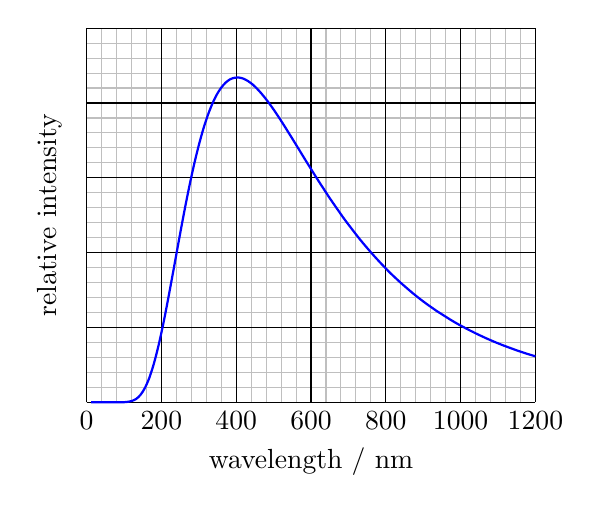
\begin{tikzpicture}[scale=1.9]
		\node[rotate=90] at (-0.25, 1.25) {relative intensity};
		\node at (1.5, -0.4) {wavelength / nm};
		\foreach \x/\xtext in {0/0, 0.5/200, 1/400, 1.5/600, 2/800, 2.5/1000, 3/1200} \node[below] at (\x, 0) {\xtext};
		\draw[thin, gray!50, step=0.1] (0,0) grid (3,2.5);
		\draw[step=0.5] (0,0) grid (3,2.5);
		\draw [blue, thick] plot [smooth] coordinates { (0.03,0) (0.06,0) (0.09,0) (0.12,0) (0.15,0) (0.18,0) (0.21,0) (0.24,0) (0.27,0.002) (0.3,0.008) (0.33,0.021) (0.36,0.049) (0.39,0.096) (0.42,0.165) (0.45,0.259) (0.48,0.376) (0.51,0.512) (0.54,0.664) (0.57,0.825) (0.6,0.989) (0.63,1.153) (0.66,1.311) (0.69,1.459) (0.72,1.596) (0.75,1.718) (0.78,1.826) (0.81,1.918) (0.84,1.994) (0.87,2.056) (0.9,2.103) (0.93,2.137) (0.96,2.159) (0.99,2.169) (1.02,2.17) (1.05,2.162) (1.08,2.146) (1.11,2.124) (1.14,2.095) (1.17,2.062) (1.2,2.025) (1.23,1.985) (1.26,1.942) (1.29,1.897) (1.32,1.85) (1.35,1.802) (1.38,1.754) (1.41,1.705) (1.44,1.656) (1.47,1.607) (1.5,1.559) (1.53,1.511) (1.56,1.464) (1.59,1.418) (1.62,1.372) (1.65,1.328) (1.68,1.285) (1.71,1.242) (1.74,1.201) (1.77,1.162) (1.8,1.123) (1.83,1.085) (1.86,1.049) (1.89,1.014) (1.92,0.98) (1.95,0.947) (1.98,0.915) (2.01,0.884) (2.04,0.854) (2.07,0.826) (2.1,0.798) (2.13,0.772) (2.16,0.746) (2.19,0.721) (2.22,0.697) (2.25,0.674) (2.28,0.652) (2.31,0.631) (2.34,0.61) (2.37,0.591) (2.4,0.572) (2.43,0.553) (2.46,0.535) (2.49,0.518) (2.52,0.502) (2.55,0.486) (2.58,0.471) (2.61,0.456) (2.64,0.442) (2.67,0.428) (2.7,0.415) (2.73,0.402) (2.76,0.39) (2.79,0.378) (2.82,0.367) (2.85,0.356) (2.88,0.345) (2.91,0.335) (2.94,0.325) (2.97,0.316) (3,0.307) };
		\end{tikzpicture}
    \vspace*{-16pt}
\end{wrapfigure}


\question{Altair, the brightest star in the constellation Aquila, is at a distance of 16.7 light years from the earth. The radiant flux intensity due to Altair measured on the earth is $1.3 \times 10^{-8} \text{ W m}^{-2}$. The intensity-wavelength curve of Altair is shown. (a) Find the luminosity of Altair. (b) Find the surface temperature of Altair. (c) Find the radius of the star.}

\subsection{cosmology}

\subsubsection{quick review: absorption spectrum} 

hot iterior of star emits a continuous range of wavelengths

as light passes cooler outer layers of the star, photons of right energies can be absorbed

the absorption depends on the elements present in the star's outer layers

this gives rise to a characteristic \emph{absorption spectrum} for the star\footnote{The chemical composition of most stars is mainly hydrogen, plus a small fraction of helium, and trace amounts of heavier elements such as carbon, oxygen, etc. The presence of each element gives rise to a unique set of absorption lines.}

the spectrum would consist of dark lines at specific wavelengths or frequencies\footnote{More detailed discussions on the absorption spectrum has been given in \S\ref{ch-atomic-spectrum}.}

\subsubsection{quick review: Doppler effect} \index{Doppler effect}

but the spectral lines observed by us will be different from where they are supposed to be

observed frequency/wavelength changes due to relative motion between star and observer

this phenomena is known as the \emph{Doppler effect}

\cmt changes in spectral lines can tell whether a star/galaxy is \emph{receding} or \emph{approaching}

\titem if wave source moves away, observed wavelength increases / frequency decreases

\titem if wave source moves closer, observed wavelength decreases / frequency increases

\cmt changes in spectral lines can also tell how fast the star is moving

you might recall observed frequency is given by: $f = f_0 \frac{c}{c \mp v}$

this formula would not be particularly useful in this part of the course

we will derive another formula for Doppler shift in the following section

\cmt Doppler shift can only tell \emph{radial} velocity of a star/galaxy

Doppler method cannot tell about motion in a dirction that is normal to line of sight

\subsubsection{redshift}

data show that spectral lines of most galaxies shift in direction of increasing wavelength

for visible spectrum, the lines shift towards red end, so this is called \keypoint{redshift}\index{redshift}

redshift of line spectrum means most galaxies are moving away

\begin{figure}[ht]
	\centering
	\begin{tikzpicture}[scale=0.85]
		\draw[thick] (2.2,0) circle (0.2);
		\draw[fill] (12,0.4) circle (0.2);
		\draw[ultra thick] (12,0.2) -- (12,-0.1) -- (11.8,-0.6) (12,-0.1) -- (12.2,-0.6) (11.75,-0.1) -- (12,0.15) -- (12.25,-0.1);
		\draw[blue,thick] (2.4, 0.62513) arc (10:-10:3.6);
		\node at (2,-1) {star};
		\node at (12,-1) {observer};
		\node at (-1.25,0) {$t=0$};
	\end{tikzpicture}
	
	\vspace*{1.5em}

	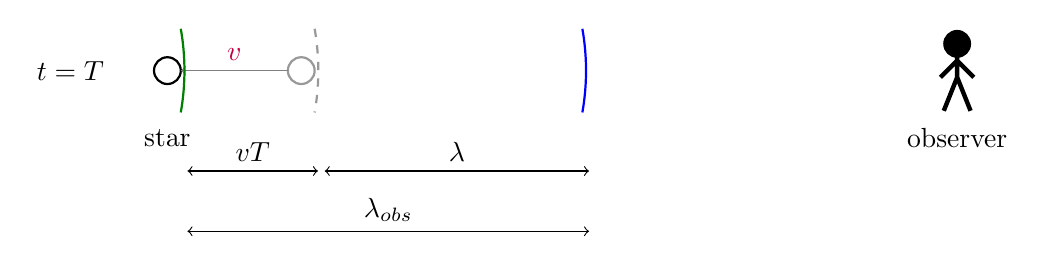
\begin{tikzpicture}[scale=0.85]
	\draw[thick] (0.2,0) circle (0.2);
	\draw[thick, gray!80] (2.2,0) circle (0.2);
	\draw[gray, <-] (0.4,0) -- (2.0,0) node[midway, above, purple]{$v$};
	\draw[fill] (12,0.4) circle (0.2);
	\draw[ultra thick] (12,0.2) -- (12,-0.1) -- (11.8,-0.6) (12,-0.1) -- (12.2,-0.6) (11.75,-0.1) -- (12,0.15) -- (12.25,-0.1);
	\draw[gray!80,dashed,thick] (2.4, 0.62513) arc (10:-10:3.6);
	\draw[blue,thick] (6.4, 0.62513) arc (10:-10:3.6);
	\draw[Green,thick] (0.4, 0.62513) arc (10:-10:3.6);
	\node at (0.2,-1) {star};
	\node at (12,-1) {observer};
	\draw[<->] (2.55,-1.5) -- (6.5,-1.5) node[above, midway]{$\lambda$};
	\draw[<->] (0.5,-1.5) -- (2.45,-1.5) node[above, midway]{$v T$};
	\draw[<->] (0.5,-2.4) -- (6.5,-2.4) node[above, midway]{$\lambda_\text{obs}$};
	\node at (-1.25,0) {$t=T$};
	\end{tikzpicture}
\end{figure}

for a star/galaxy recedes at velocity $v$, it travels a distance of $v T$ in one period

this causes an increase in observed wavelength: $\Delta \lambda = \lambda_\text{obs} - \lambda = v T$

so fractional change in wavelength is: $\frac{\Delta \lambda}{\lambda} = \frac{vT}{\lambda} = \frac{vT}{cT} \RA \boxed{z \equiv \frac{\Delta \lambda}{\lambda} = \frac{v}{c}}$

the parameter $z$ is usually called the \emph{redshift factor}


\subsubsection{recession of galaxies}

\emph{Edwin Hubble} discovered in 1929 that almost all galaxies are moving away

further analysis showed recession speed of a galaxy is roughly proportional to its distance

\begin{figure}[ht]
    \centering
    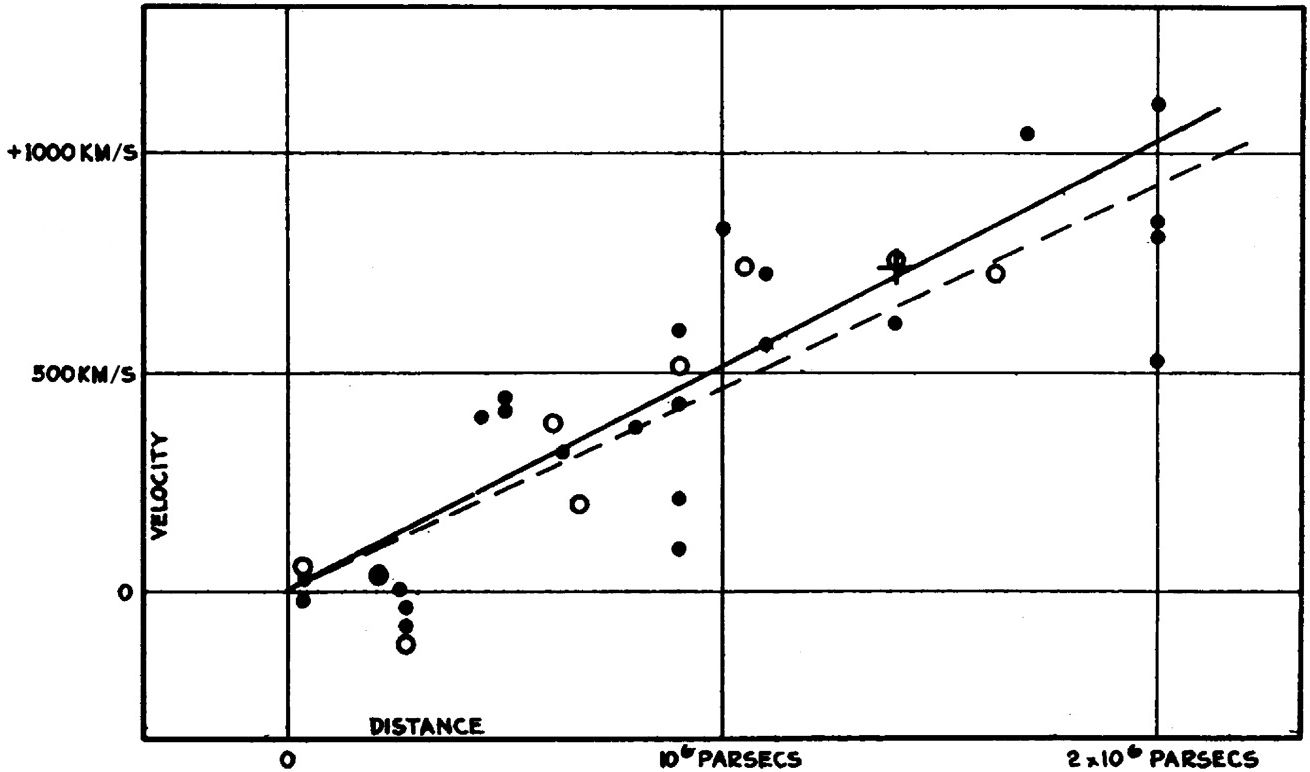
\includegraphics[width=0.8\textwidth]{pnas-168fig.jpeg}

	Edwin Hubble's plot of the velocity-distance relation among galaxies in his original paper
	\vspace*{-12pt}
\end{figure}


this\index{Hubble's law} is known as \keypoint{Hubble's law}\footnote{Edwin Hubble made this conclusion based on his study of 46 galaxies. Later observations further supported the proportional relationship between the recession speed of galaxies and the distance, but the constant computed by Edwin Hubble himself was found to be greatly overestimated. Hubble's original paper can be seen here: \url{https://www.pnas.org/doi/full/10.1073/pnas.15.3.168}}
\begin{equation*}
	\boxed{v = H_0 d} \qquad \text{ Hubble constant: } H_0 \approx 2.4 \times10^{-18} \text{ s}^{-1}
\end{equation*}

\cmt exact value of the Hubble constant is not accurately known

$H_0$ is believed to be between $1.5 \times10^{-18} \text{ s}^{-1} \sim 3.5 \times10^{-18}\text{ s}^{-1}$ (uncertainty around $\pm 40\%$!)


\example{The K-line of inoised calcium from the absorption spectrum of the galaxy NGC 4889 is measured to be 401.8 nm. The same K-line measured in a laboratory setting is known to be 393.3 nm. (a) What is the speed of the NGC 4889? (b) How long does it take for light to reach us from NGC 4889?}

\sol recession speed: $v = \frac{\Delta \lambda}{\lambda} \times c = \frac{401.8-393.3}{393.3}\times 3.00\times10^8 \approx 6.48 \times 10^6 \mps$

distance of galaxy: $d = \frac{v}{H_0} \approx \frac{6.48\times10^6}{2.4\times10^{-18}} \approx 2.7 \times 10^{24} \text{ m}$

time for light to propagate: $t = \frac{d}{c} = \frac{2.7 \times 10^{24}}{3.00\times10^8} \approx 9.0\times10^{15} \text{ s} \approx 2.9\times10^{8} \text{ years}$

\subsubsection{Big Bang theory}\index{Big Bang}

Hubble's law implies the universe is \emph{expanding}

go back in time, all galaxies must be close together

this suggests the universe must begin from a highly dense state

it is now generally accepted that the universe is created from a dramatic explosion

this starting point of the universe and everything is known as the \keypoint{Big Bang}\footnote{The Big Bang Theory was proposed in 1927 by Belgian astronomer and cosmologist \emph{Georges Lemaitre}. From a theoretical view, Lemaitre deduced that the natural consequence of Einstein's theory of general relativity must be an expanding universe. In 1929, \emph{Edwin Hubble}, who was unaware of Lemaitre's work, published his famous relation between distance and radial velocity among extra-galactic nebulae. Nevertheless, Hubble's discovery became a strong supporting evidence for the Big Bang theory.}

\subsubsection*{age of the universe}

age of the universe can be deduced from Hubble's law

consider two galaxies started off close together during the Big Bang

assume galaxies have been moving away from one another at constant speed $v$ for time $t$

distance between the two galaxies today would be $d=vt$

but this $t$ is essentially all the time since beginning of the universe

so age of the universe: $t=\frac{d}{v} = \frac{d}{H_0 d} \RA \boxed{ t= \frac{1}{H_0}}$

substitute $H_0 \approx 2.4 \times10^{-18} \text{ s}^{-1}$, one finds $t\approx 4.5\times10^{18} \text{ s}$, which is about 14 billion years (Gy)

\cmt there is great uncertainty in the universe's age (varying from $11\sim20 \text{ Gy}$)

two main reasons for this uncertainty are:

\begin{compactitem}

\item[--] our calculation is based on the assumption of constant recession speed

there are cosmological models that suggest otherwise, so different ages are predicted 

\item[--] our calculation also depends on the value of $H_0$

but exact value of $H_0$ is in doubt due to large uncertainty in distance measurements

\end{compactitem}


\begin{wrapfigure}{r}{0.52\textwidth}
    \vspace*{-15pt}
    \centering
	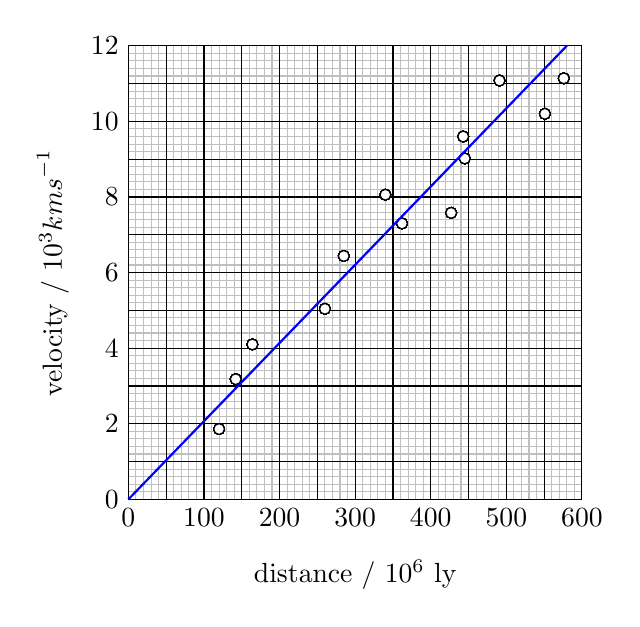
\begin{tikzpicture}[scale=0.96]
		\node[rotate=90] at (-1, 3) {velocity / $10^3 \text{ km s}^{-1}$};
		\node at (3, -1) {distance / $10^6$ ly};
		\foreach \y/\ytext in {0/0, 1/2, 2/4, 3/6, 4/8, 5/10, 6/12} \node[left] at (0,\y) {\ytext};
		\foreach \x/\xtext in {0/0, 1/100, 2/200, 3/300, 4/400, 5/500, 6/600} \node[below] at (\x, 0) {\xtext};
		\draw[thin, gray!50, step=0.1] (0,0) grid (6,6);
		\draw[step=0.5] (0,0) grid (6,6);
		\draw plot[mark=*, mark options={fill=white}] (1.20, 0.93);
		\draw plot[mark=*, mark options={fill=white}] (1.42, 1.59);
		\draw plot[mark=*, mark options={fill=white}] (1.64, 2.05);
		\draw plot[mark=*, mark options={fill=white}] (2.60, 2.52);
		\draw plot[mark=*, mark options={fill=white}] (2.85, 3.22);
		\draw plot[mark=*, mark options={fill=white}] (3.40, 4.03);
		\draw plot[mark=*, mark options={fill=white}] (3.62, 3.65);
		\draw plot[mark=*, mark options={fill=white}] (4.27, 3.79);
		\draw plot[mark=*, mark options={fill=white}] (4.43, 4.80);
		\draw plot[mark=*, mark options={fill=white}] (4.45, 4.51);
		\draw plot[mark=*, mark options={fill=white}] (4.91, 5.54);
		\draw plot[mark=*, mark options={fill=white}] (5.51, 5.10);
		\draw plot[mark=*, mark options={fill=white}] (5.76, 5.57);
		\draw[thick, blue] (0,0) -- (5.8, 6);
		\end{tikzpicture}
    \vspace*{-18pt}
\end{wrapfigure}

\question{The plot shows some data on the velocities and distances for a set of galaxies. A fit line has also been drawn. (a) Compute a value for the Hubble constant $H_0$ based on the data given. (b) Estimate the age of the universe using your calculated value for $H_0$, and state any assumption that you make. (c) For a galaxy at a distance of $2\times10^9 \text{ ly}$, what is the fractional change in the wavelength of its spectrum?}



\subsubsection*{cosmic microwave background radiation}\index{comsmic microwave background}

another key evidence for the Big Bang model is the \emph{cosmic microwave background}

after Big Bang, universe gradually cools down due to expansion

the universe today should be filled with radiation due to remnant heat from the Big Bang

theoretical calculation predicts that the universe should now have a temperature of 2.7 K

this suggests a background radiation peaked at around 1 mm (microwave band)

this radiation is therefore called \keypoint{cosmic microwave background} (CMB)\footnote{\emph{Ralph Alpher}, \emph{George Gamow} and \emph{Robert Herman} suggested the idea of CMB in theory in the 1940s. In 1965, \emph{Robert Dicke} took up the problem and led a team of physicists at Princeton University to hunt for the CMB signal. In the same year, \emph{Arno Penzias} and \emph{Robert Wilson} at the Bell Laboratories built a large radio antenna for a communication satellite in New Jersey, while they failed in all attempts to get rid of the `background noise' that came from all directions.

When Princeton's team heard about the Bell Lab's result, they realized at once that the CMB had already been found. As a result, two important articles were published: one by Penzias and Wilson about the `noise', the other by Dicke's team explaining its true nature. Penzias and Wilson did not interpret what they had found in their article, nor did they have any intention to look for CMB in the first place. Nevertheless, they received the Nobel Prize in Physics in 1978, for their accidental discovery of CMB. What about Dicke and his team? Quoting \emph{Bill Bryson's A Short History of Nearly Everything}, the Princeton researchers got only sympathy.}

CMB radiation have been observed by space telescopes from all directions of cosmos\footnote{Three major CMB missions include: (1) the Cosmic Background Explorer (COBE), launched by NASA in 1989, (2) the Wilkinson Microwave Anisotropy Probe (WMAP), launched by NASA in 2001 to study fluctuations in CMB in greater detail, (3) the Planck satellite, launched by ESA in 2009 to study CMB fluctuations with even greater sensitivity. These studies would allow scientists to trace back to what happened immediately after the Big Bang, and the understanding of the early universe is crucial for the understanding of the large-scale cosmic structures that we see today.}

CMB corresponds to a temperature of around 3 K, which is pretty close to the prediction

 \question{Use Wien's law to show that the peak intensity of the electromagnetic radiation given off by a black body at a temperature of 3 K is around 1 mm.}


\subsubsection{fate of the universe ($\ast$)}

whether the universe will expand forever depends on strength of gravity

fate of universe narrows down to how density $\rho$ of universe compares to critical density $\rho_c$

\begin{compactitem}

\item[--] if $\rho > \rho_c$, force of gravity dominates as there is sufficient matter

expansion will slow down, then contract back inwards

this leads to a \emph{closed} universe, eventually ending in a \emph{Big Crunch} 

\item[--] if $\rho < \rho_c$, there is not enough gravity to stop expansion

expansion continues forever, leading to an \emph{open} universe

\end{compactitem}

but the big problem is, it is difficult to determine average density of our universe

\cmt issue of \emph{dark matter}\index{dark matter}

mass of galaxies suggested by luminosity calculation cannot provide the centripetal force needed to keep galaxies rotating

galaxies must contain mass that does not give off light, known as \keypoint{dark matter}

\cmt issue of \emph{dark energy}\index{dark energy}

observation shows expansion of universe is not slowing down

it is suggested that cosmic acceleration is caused by \keypoint{dark energy}

\begin{figure}[ht]
    \centering
	\begin{tikzpicture}
		\draw[thick] (0,0) circle (2);
		\draw[thick] (0,0) -- (68:2);
		\draw[thick] (0,0) -- (165.2:2);
		\draw[thick] (0,0) -- (50:2);
		\draw[thick] (58.8:1.8) --++ (1,0.5) node[right, twolinecap] {ordinary matter\\5\%};
		\draw[thick] (-40:1.7) --++ (1.1,-0.6) node[right, twolinecap] {dark energy\\68\%};
		\draw[thick] (120:1.8) --++ (-1,0.6) node[left, twolinecap] {dark matter\\27\%};
    \end{tikzpicture}
    \vspace*{-12pt}
\end{figure}


\cmt it turns out ordinary matter only contributes to a very small part of the universe

great majority of the total mass-energy content of cosmos is dark matter and dark energy

but nature of dark matter and dark energy are not yet understood